\documentclass{standalone}
% \documentclass{article}

\usepackage{tikz}

\begin{document}

\begin{tikzpicture}

\onslide<1->{\node[text=red!70!black] at (0, 1.2) {\scalebox{0.6}{\tiny{\texttt{fig, axarr = plt.subplots(2, 2)}}}};}
\onslide<2>{\node at (0, 0) {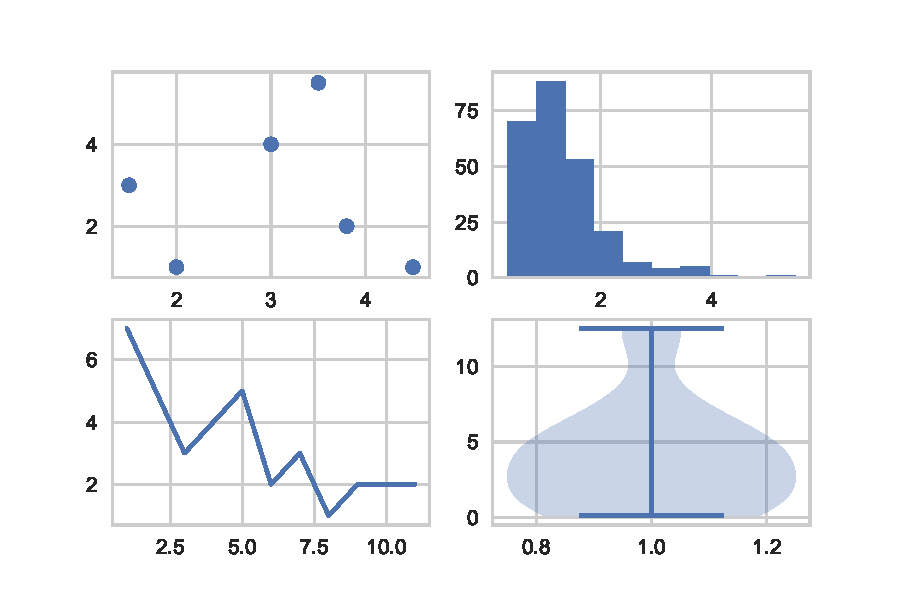
\includegraphics[width=0.3\textwidth]{../subplot_demo.pdf}};}
\onslide<3->{
\node[opacity=0.3] at (0, 0) {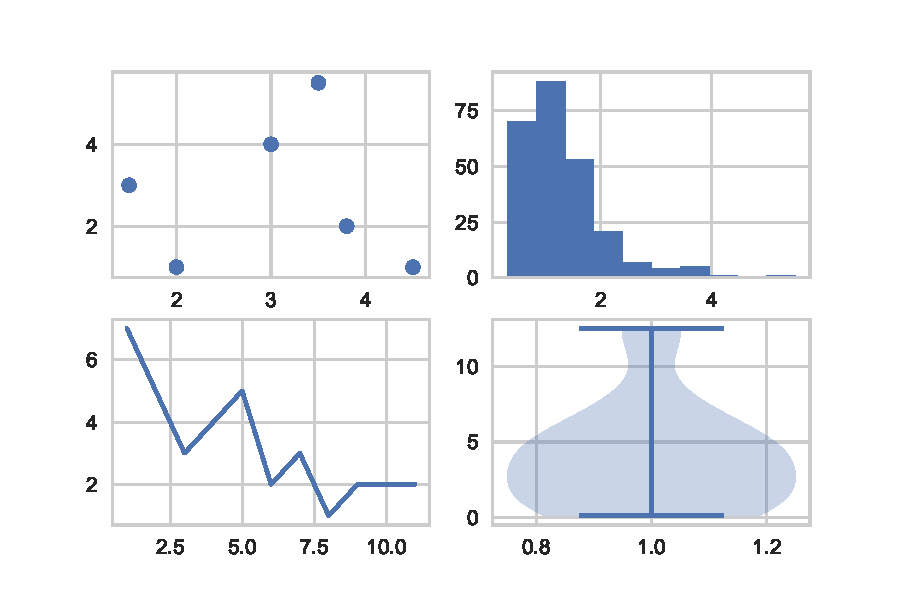
\includegraphics[width=0.3\textwidth]{../subplot_demo.pdf}};
\node[text=red!70!black] at (-0.625, 0.45) {\scalebox{0.45}{\tiny{\texttt{axarr[0, 0].scatter()}}}};
\node[text=red!70!black] at (0.725, 0.45) {\scalebox{0.45}{\tiny{\texttt{axarr[0, 1].hist()}}}};
\node[text=red!70!black] at (-0.65, -0.45) {\scalebox{0.45}{\tiny{\texttt{axarr[1, 0].plot()}}}};
\node[text=red!70!black] at (0.725, -0.45) {\scalebox{0.45}{\tiny{\texttt{axarr[1, 1].violinplot()}}}};
}

\end{tikzpicture}

\end{document}
